% Options for packages loaded elsewhere
\PassOptionsToPackage{unicode}{hyperref}
\PassOptionsToPackage{hyphens}{url}
\PassOptionsToPackage{dvipsnames,svgnames,x11names}{xcolor}
%
\documentclass[
  letterpaper,
  DIV=11,
  numbers=noendperiod]{scrartcl}

\usepackage{amsmath,amssymb}
\usepackage{iftex}
\ifPDFTeX
  \usepackage[T1]{fontenc}
  \usepackage[utf8]{inputenc}
  \usepackage{textcomp} % provide euro and other symbols
\else % if luatex or xetex
  \usepackage{unicode-math}
  \defaultfontfeatures{Scale=MatchLowercase}
  \defaultfontfeatures[\rmfamily]{Ligatures=TeX,Scale=1}
\fi
\usepackage{lmodern}
\ifPDFTeX\else  
    % xetex/luatex font selection
\fi
% Use upquote if available, for straight quotes in verbatim environments
\IfFileExists{upquote.sty}{\usepackage{upquote}}{}
\IfFileExists{microtype.sty}{% use microtype if available
  \usepackage[]{microtype}
  \UseMicrotypeSet[protrusion]{basicmath} % disable protrusion for tt fonts
}{}
\makeatletter
\@ifundefined{KOMAClassName}{% if non-KOMA class
  \IfFileExists{parskip.sty}{%
    \usepackage{parskip}
  }{% else
    \setlength{\parindent}{0pt}
    \setlength{\parskip}{6pt plus 2pt minus 1pt}}
}{% if KOMA class
  \KOMAoptions{parskip=half}}
\makeatother
\usepackage{xcolor}
\setlength{\emergencystretch}{3em} % prevent overfull lines
\setcounter{secnumdepth}{5}
% Make \paragraph and \subparagraph free-standing
\ifx\paragraph\undefined\else
  \let\oldparagraph\paragraph
  \renewcommand{\paragraph}[1]{\oldparagraph{#1}\mbox{}}
\fi
\ifx\subparagraph\undefined\else
  \let\oldsubparagraph\subparagraph
  \renewcommand{\subparagraph}[1]{\oldsubparagraph{#1}\mbox{}}
\fi


\providecommand{\tightlist}{%
  \setlength{\itemsep}{0pt}\setlength{\parskip}{0pt}}\usepackage{longtable,booktabs,array}
\usepackage{calc} % for calculating minipage widths
% Correct order of tables after \paragraph or \subparagraph
\usepackage{etoolbox}
\makeatletter
\patchcmd\longtable{\par}{\if@noskipsec\mbox{}\fi\par}{}{}
\makeatother
% Allow footnotes in longtable head/foot
\IfFileExists{footnotehyper.sty}{\usepackage{footnotehyper}}{\usepackage{footnote}}
\makesavenoteenv{longtable}
\usepackage{graphicx}
\makeatletter
\def\maxwidth{\ifdim\Gin@nat@width>\linewidth\linewidth\else\Gin@nat@width\fi}
\def\maxheight{\ifdim\Gin@nat@height>\textheight\textheight\else\Gin@nat@height\fi}
\makeatother
% Scale images if necessary, so that they will not overflow the page
% margins by default, and it is still possible to overwrite the defaults
% using explicit options in \includegraphics[width, height, ...]{}
\setkeys{Gin}{width=\maxwidth,height=\maxheight,keepaspectratio}
% Set default figure placement to htbp
\makeatletter
\def\fps@figure{htbp}
\makeatother

\KOMAoption{captions}{tableheading}
\makeatletter
\makeatother
\makeatletter
\makeatother
\makeatletter
\@ifpackageloaded{caption}{}{\usepackage{caption}}
\AtBeginDocument{%
\ifdefined\contentsname
  \renewcommand*\contentsname{Table of contents}
\else
  \newcommand\contentsname{Table of contents}
\fi
\ifdefined\listfigurename
  \renewcommand*\listfigurename{List of Figures}
\else
  \newcommand\listfigurename{List of Figures}
\fi
\ifdefined\listtablename
  \renewcommand*\listtablename{List of Tables}
\else
  \newcommand\listtablename{List of Tables}
\fi
\ifdefined\figurename
  \renewcommand*\figurename{Figure}
\else
  \newcommand\figurename{Figure}
\fi
\ifdefined\tablename
  \renewcommand*\tablename{Table}
\else
  \newcommand\tablename{Table}
\fi
}
\@ifpackageloaded{float}{}{\usepackage{float}}
\floatstyle{ruled}
\@ifundefined{c@chapter}{\newfloat{codelisting}{h}{lop}}{\newfloat{codelisting}{h}{lop}[chapter]}
\floatname{codelisting}{Listing}
\newcommand*\listoflistings{\listof{codelisting}{List of Listings}}
\makeatother
\makeatletter
\@ifpackageloaded{caption}{}{\usepackage{caption}}
\@ifpackageloaded{subcaption}{}{\usepackage{subcaption}}
\makeatother
\makeatletter
\@ifpackageloaded{tcolorbox}{}{\usepackage[skins,breakable]{tcolorbox}}
\makeatother
\makeatletter
\@ifundefined{shadecolor}{\definecolor{shadecolor}{rgb}{.97, .97, .97}}
\makeatother
\makeatletter
\makeatother
\makeatletter
\makeatother
\ifLuaTeX
  \usepackage{selnolig}  % disable illegal ligatures
\fi
\IfFileExists{bookmark.sty}{\usepackage{bookmark}}{\usepackage{hyperref}}
\IfFileExists{xurl.sty}{\usepackage{xurl}}{} % add URL line breaks if available
\urlstyle{same} % disable monospaced font for URLs
\hypersetup{
  pdftitle={Projet d'Analyse des Données Économiques avec R},
  pdfauthor={Haithem Farjallah et Omar Majri},
  colorlinks=true,
  linkcolor={blue},
  filecolor={Maroon},
  citecolor={Blue},
  urlcolor={Blue},
  pdfcreator={LaTeX via pandoc}}

\title{Projet d'Analyse des Données Économiques avec R}
\author{Haithem Farjallah et Omar Majri}
\date{}

\begin{document}
\maketitle
\ifdefined\Shaded\renewenvironment{Shaded}{\begin{tcolorbox}[interior hidden, boxrule=0pt, borderline west={3pt}{0pt}{shadecolor}, sharp corners, breakable, frame hidden, enhanced]}{\end{tcolorbox}}\fi

\renewcommand*\contentsname{Table of contents}
{
\hypersetup{linkcolor=}
\setcounter{tocdepth}{3}
\tableofcontents
}
\hypertarget{i.-introduction}{%
\section{I. Introduction}\label{i.-introduction}}

\hypertarget{description-du-projet}{%
\subsection{Description du Projet}\label{description-du-projet}}

Notre projet tourne autour de la collecte, du nettoyage, de l'analyse et
de la visualisation des données économiques en utilisant R. Nous avons
choisi de nous concentrer sur des ensembles de données liés à des
entreprises de renom telles qu'Amazon, Microsoft et d'autres, car elles
offrent des informations précieuses sur le paysage économique. Nous
explorerons divers indicateurs économiques, tendances et modèles pour
extraire des insights significatifs pouvant éclairer les processus de
prise de décision.

\hypertarget{collecte-des-donnuxe9es}{%
\section{Collecte des Données}\label{collecte-des-donnuxe9es}}

\hypertarget{source-des-donnuxe9es-yahoo-finance---les-plus-actifs}{%
\subsection{Source des données : Yahoo Finance - Les plus
actifs}\label{source-des-donnuxe9es-yahoo-finance---les-plus-actifs}}

Les données utilisées dans ce projet proviennent de la page ``Les plus
actifs'' de Yahoo Finance. Cette source fournit une liste complète des
actions les plus échangées, comprenant des détails tels que la date, les
prix d'ouverture, de clôture, les plus hauts et les plus bas, ainsi que
le volume de transactions et le nom de l'entreprise associée.

\hypertarget{ii.-netoyage-des-donuxe9es}{%
\subsection{II. Netoyage des donées
:}\label{ii.-netoyage-des-donuxe9es}}

\begin{enumerate}
\def\labelenumi{\arabic{enumi}.}
\item
  \textbf{Vérification des valeurs manquantes :}

  Nous avons commencé par vérifier et supprimer les lignes contenant des
  valeurs manquantes à l'aide de la fonction
  \textbf{\texttt{complete.cases}}. Cela garantit l'intégrité de nos
  données en éliminant les observations incomplètes.
\item
  \textbf{Vérification du format de la date :}

  Ensuite, nous avons utilisé la bibliothèque lubridate pour confirmer
  que la colonne `Date' était au bon format de date, et nous avons
  converti cette colonne en format de date avec
  \textbf{\texttt{as.Date}}. Cela assure la cohérence dans la gestion
  des dates pour nos analyses ultérieures.
\item
  \textbf{Vérification des valeurs négatives :}

  Nous avons également vérifié qu'il n'y avait pas de valeurs négatives
  dans les colonnes numériques pertinentes telles que `Open', `High',
  `Low', `Close', `Adj.Close', et `Volume'.
\item
  \textbf{Vérification de la cohérence des valeurs `High' et `Low' :}

  Une étape cruciale a été de garantir la cohérence des données en
  vérifiant que les valeurs dans la colonne `High' étaient toujours
  supérieures ou égales aux valeurs correspondantes dans la colonne
  `Low'.
\item
  \textbf{Résumé statistique des données nettoyées :}

  Après ce nettoyage initial, nous avons généré un résumé statistique
  pour la colonne `Close', ce qui nous a donné un aperçu des propriétés
  centrales et de la dispersion de nos données.

  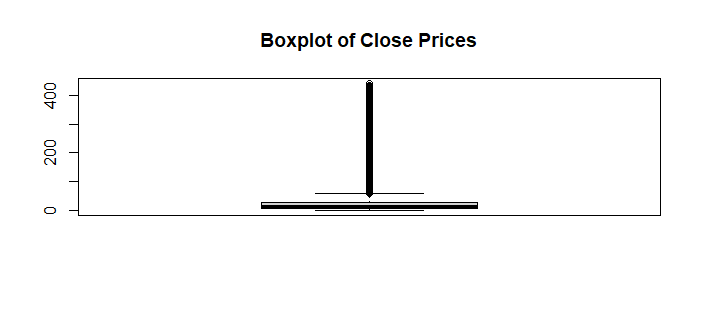
\includegraphics{images/boxplotClosePrices.png}
\item
  \textbf{Visualisation des valeurs aberrantes (outliers) :}

  Pour détecter et traiter les valeurs aberrantes, nous avons créé un
  diagramme en boîte pour visualiser la distribution des prix de clôture
  après le nettoyage. Cela nous a permis de mieux comprendre et gérer
  les valeurs extrêmes qui pourraient affecter nos analyses.

  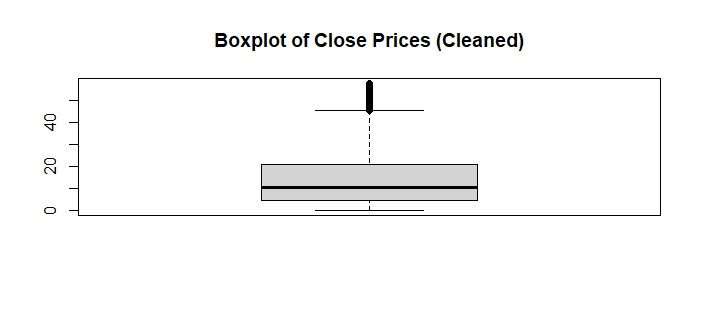
\includegraphics{images/boxplotClosePriceCleaned.png}
\end{enumerate}

\hypertarget{iii.analyse-des-donnees}{%
\section{III.Analyse des donnees}\label{iii.analyse-des-donnees}}

\begin{enumerate}
\def\labelenumi{\arabic{enumi}.}
\item
  \textbf{Chargement des bibliothèques nécessaires :}

  Nous avons commencé par charger les bibliothèques essentielles telles
  que ggplot2, lmtest et dplyr pour effectuer nos analyses et
  visualisations.
\item
  \textbf{Conversion de la colonne ``Date'' :}

  Nous avons converti la colonne ``Date'' en type de données Date pour
  faciliter la manipulation temporelle de nos données.
\item
  \textbf{Filtrage des données :} Les données ont été filtrées pour
  inclure uniquement les sociétés sélectionnées et les données des six
  derniers mois, ce qui nous a permis de nous concentrer sur des données
  récentes et pertinentes.
\item
  \textbf{Création de graphiques individuels :}

  Des graphiques ont été créés pour chaque société sélectionnée,
  montrant l'évolution du prix de clôture et du volume de ventes,
  offrant ainsi une perspective visuelle sur les performances des
  entreprises étudiées.

  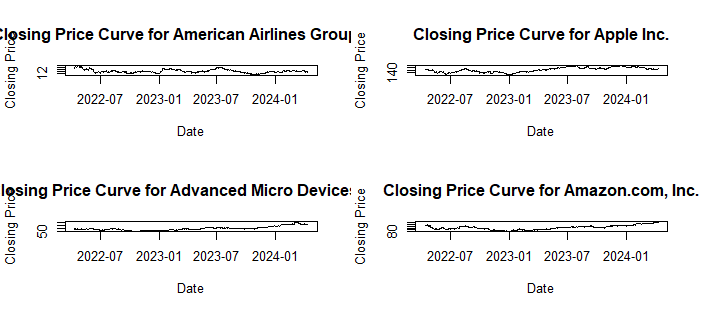
\includegraphics{images/ClosingPriceCurevCompanies.png}

  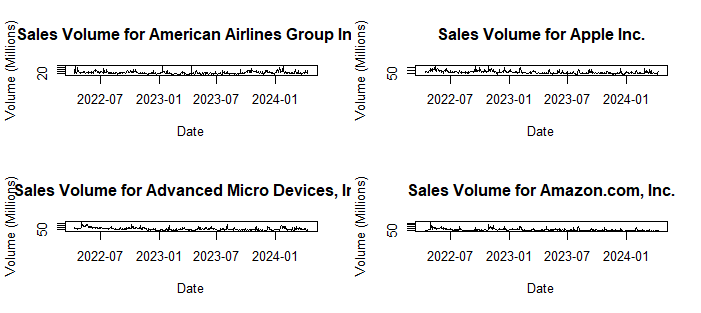
\includegraphics{images/SlaesVolumeCompanies.png}
\item
  \textbf{Calcul des moyennes mobiles :}

  Nous avons calculé les moyennes mobiles pour chaque société et
  représenté graphiquement les prix de clôture ajustés et les moyennes
  mobiles pour observer les tendances à long terme.
\end{enumerate}

\texttt{A.American\ Airlines\ Group\ Inc\ :}

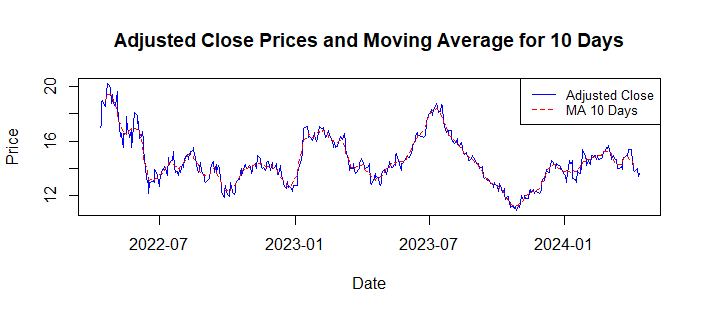
\includegraphics{images/MovingAverage10daysUS.png}

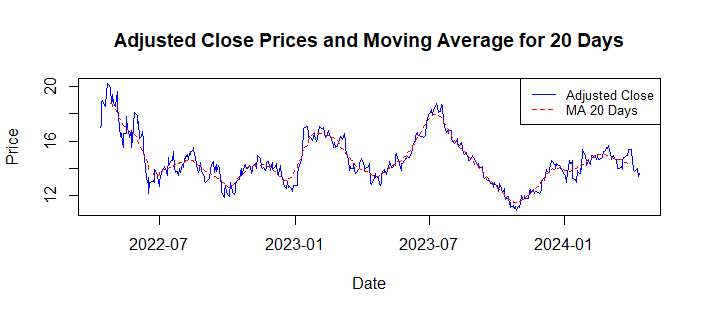
\includegraphics{images/MovingAverage20DaysUS.png}

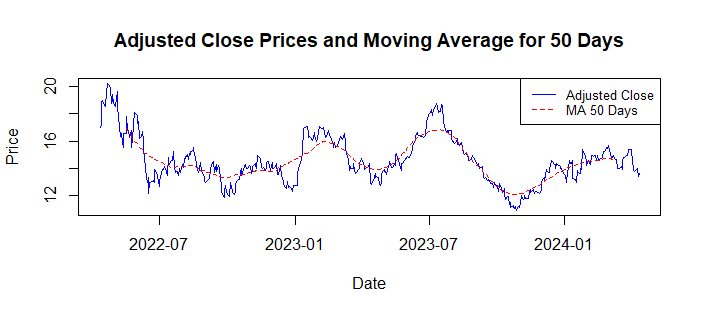
\includegraphics{images/MovingAverage50daysUS.png}

\texttt{B.Apple\ Inc\ :}

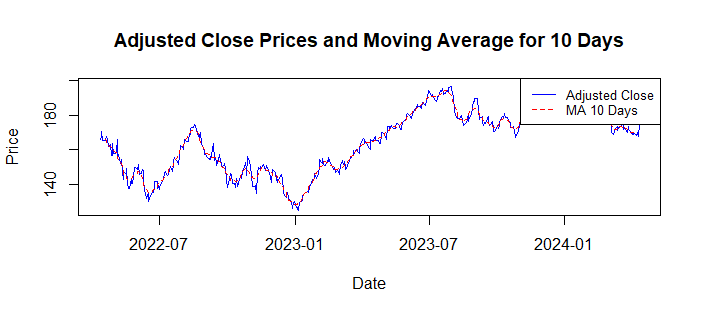
\includegraphics{images/MovingAverage10daysApple.png}

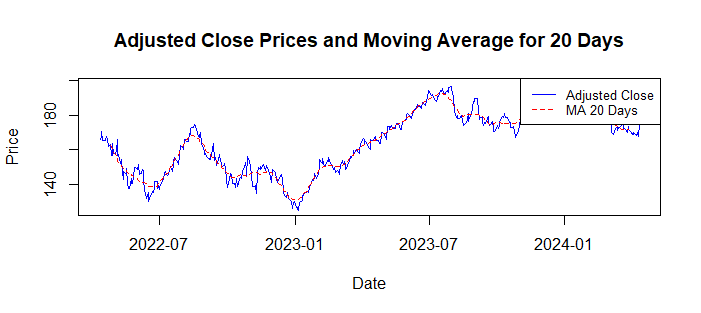
\includegraphics{images/MovingAverage20daysApple.png}

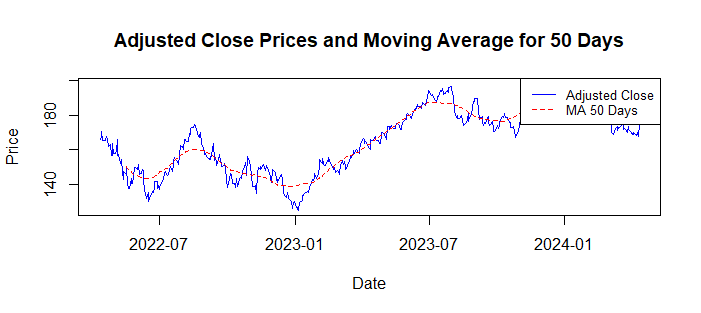
\includegraphics{images/MovingAverage50daysApple.png}

\texttt{C.Advanced\ Micro\ Devices,\ Inc\ :}

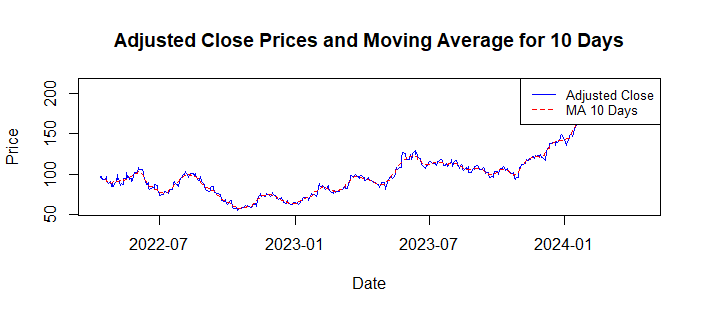
\includegraphics{images/MovingAverage10daysMD.png}

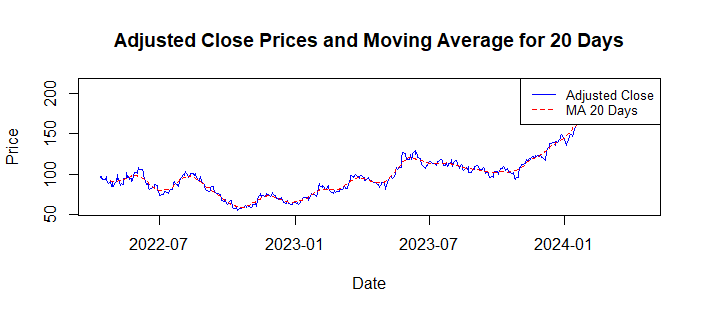
\includegraphics{images/MovingAverage20daysMD.png}

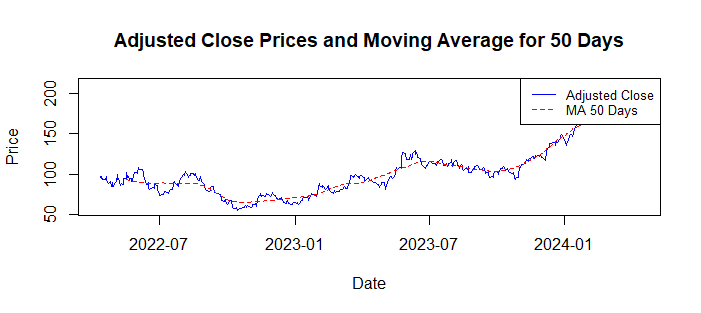
\includegraphics{images/MovingAverage50daysMD.png}

\texttt{D.Amazon.com,\ Inc\ :}

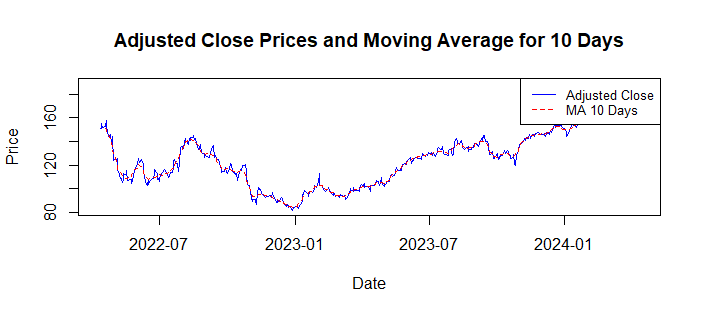
\includegraphics{images/MovingAverage10daysAmazon.png}

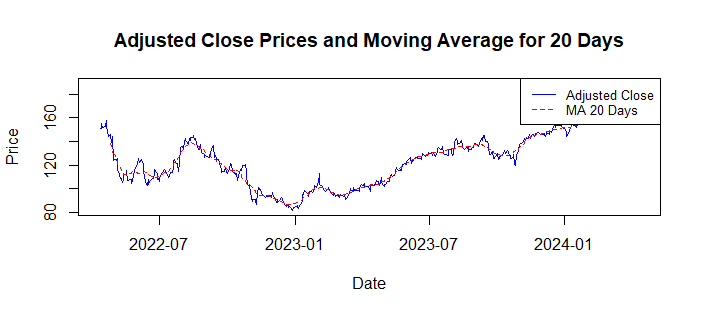
\includegraphics{images/MovingAverage20daysAmazon.png}

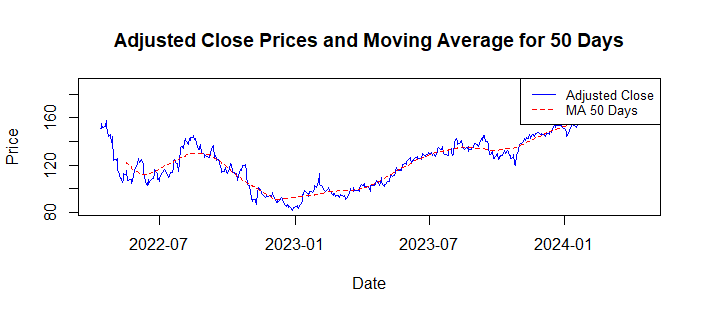
\includegraphics{images/MovingAverage50daysAmazon.png}

\begin{enumerate}
\def\labelenumi{\arabic{enumi}.}
\setcounter{enumi}{6}
\tightlist
\item
  \textbf{Calcul de la corrélation :} En calculant la corrélation entre
  les prix d'ouverture et de clôture, ainsi qu'entre les prix les plus
  élevés et les prix les plus bas, nous avons pu visualiser ces
  relations à l'aide de graphiques de dispersion, ce qui nous a donné
  des informations sur les liens entre différentes variables.
\end{enumerate}

\includegraphics{images/correlationOpen\&Close.png}

\includegraphics{images/relationOpen\&Close.png}

\texttt{corrélation\ entre\ les\ prix\ les\ plus\ élevés\ et\ les\ prix\ les\ plus\ bas\ :}

\includegraphics{images/correlationHigh\&low.png}

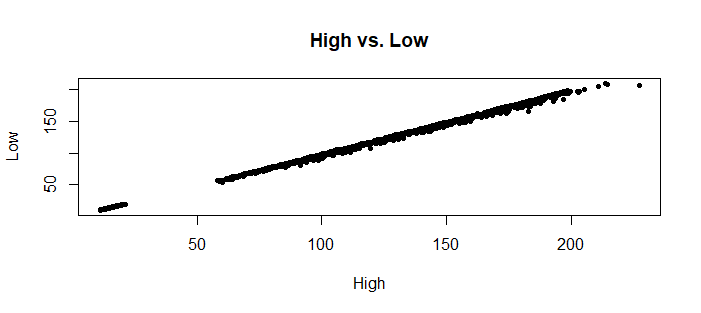
\includegraphics{images/HighvsLow.png}

\begin{enumerate}
\def\labelenumi{\arabic{enumi}.}
\setcounter{enumi}{7}
\tightlist
\item
  \textbf{Groupement et analyse du volume des ventes :} Nous avons
  groupé les données par société pour calculer le volume total des
  ventes et identifier les dix sociétés ayant le volume le plus élevé au
  cours des six derniers mois, ce qui est essentiel pour comprendre
  l'activité économique de ces entreprises.
\end{enumerate}

\begin{figure}

{\centering 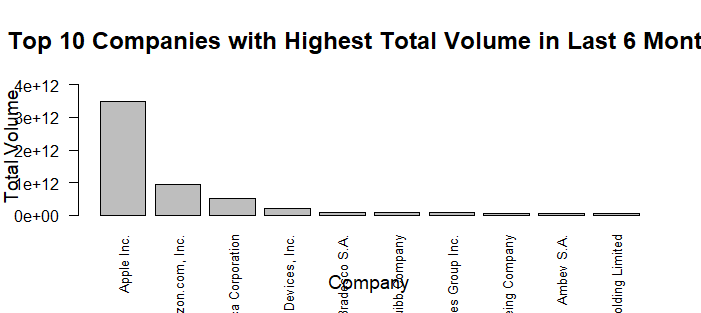
\includegraphics[width=5.5625in,height=\textheight]{images/top10Companies.png}

}

\end{figure}

\hypertarget{iii.-prediction}{%
\section{III. Prediction :}\label{iii.-prediction}}

\begin{enumerate}
\def\labelenumi{\arabic{enumi}.}
\item
  \textbf{Filtrage des données pour AMD :}

  Les données ont été filtrées pour inclure uniquement les entrées liées
  à AMD, une étape préalable à la prédiction spécifique pour cette
  entreprise.
\item
  \textbf{Imputation des valeurs manquantes :}

  Nous avons remplacé les valeurs manquantes dans la colonne ``Close''
  par la moyenne des valeurs disponibles pour AMD, assurant ainsi la
  continuité des données nécessaires à la prédiction.
\item
  \textbf{Ingénierie des fonctionnalités :}

  En créant des variables retardées basées sur les prix de clôture
  antérieurs, nous avons préparé nos données pour l'entraînement du
  modèle de prédiction.
\item
  \textbf{Division des données et définition des caractéristiques :}

  Les données ont été divisées en ensembles d'entraînement et de test,
  avec la définition des caractéristiques à utiliser pour la prédiction
  et la variable cible, à savoir les prix de clôture.
\item
  \textbf{Entraînement du modèle et évaluation :}

  Un modèle de forêt aléatoire a été entraîné en utilisant les données
  d'entraînement, puis utilisé pour prédire les prix de clôture sur les
  données de test. Enfin, les métriques de précision telles que MAE, MSE
  et RMSE ont été calculées pour évaluer la performance du modèle.
\item
  \textbf{Visualisation des prédictions :}

  Les valeurs réelles et prédites des prix de clôture ont été
  visualisées sur un graphique pour comparer les prédictions au
  comportement réel, offrant ainsi une évaluation visuelle de
  l'efficacité de notre modèle de prédiction.

  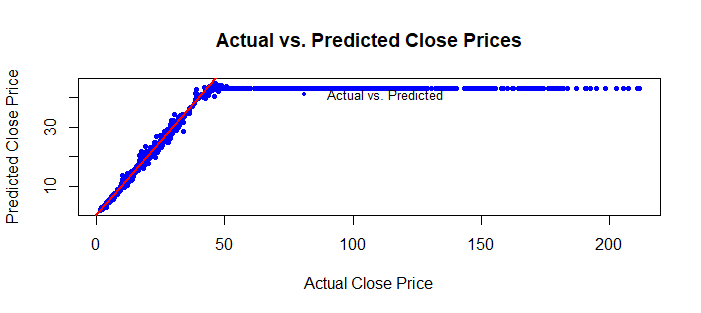
\includegraphics{images/ActualVSPredictClosePrices.png}
\end{enumerate}



\end{document}
